\documentclass{article}
\usepackage{amsmath,amssymb,amsthm,kotex,mdframed,paralist}

\newcounter{num}
%\newcommand{\defi}[1]
%{\bigskip\noindent\refstepcounter{num}\textbf{정의 \arabic{num}) #1}\par}
%\newcommand{\theo}[1]
%{\bigskip\noindent\refstepcounter{num}\textbf{정리 \arabic{num}) #1}\par}
\newcommand{\exam}[1]
{\bigskip\noindent\refstepcounter{num}\textbf{예제 \arabic{num}) #1}\par}
\newcommand{\prob}[1]
{\bigskip\noindent\refstepcounter{num}\textbf{문제 \arabic{num}) #1}\par}
\newcommand{\summ}[1]
{\bigskip\noindent\refstepcounter{num}\textbf{요약 \arabic{num}) #1}\par}

\renewcommand{\figurename}{그림}
%\renewcommand{\proofname}{증명)}
\newcommand{\sol}{\par\bigskip\noindent{\bfseries풀이)}\par}
\newcommand{\ans}[1]{{\raggedleft\textbf{답 : }#1\par}}

\addtolength{\oddsidemargin}{-.875in}
	\addtolength{\evensidemargin}{-.875in}
	\addtolength{\textwidth}{1.75in}

	\addtolength{\topmargin}{-.875in}
	\addtolength{\textheight}{1.75in}
%%%
\begin{document}

\title{성민 : 02 확률과 통계[자이스토리] 관련 문제들}
\author{}
\date{\today}
\maketitle
%\tableofcontents

%
\prob{B36-1}
그림은 합동인 정사각형 15개를 연결하여 만든 도형을 나타낸 것이다.
이 도형의 선들로 이루어질 수 있는 직사각형의 개수는?
\begin{figure}[h!]
\centering
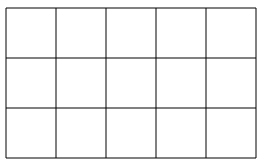
\includegraphics[width=0.3\textwidth]{B36-1}
\end{figure}

%
\prob{B36-2}
그림은 합동인 정사각형 11개를 연결하여 만든 도형을 나타낸 것이다.
이 도형의 선들로 이루어질 수 있는 직사각형의 개수는?
\begin{figure}[h!]
\centering
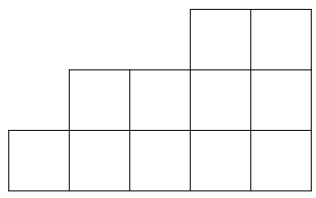
\includegraphics[width=0.3\textwidth]{B36-2}
\end{figure}

%
\prob{B36-3}
그림은 합동인 정사각형 12개를 연결하여 만든 도형을 나타낸 것이다.
이 도형의 선들로 이루어질 수 있는 직사각형의 개수는?
\begin{figure}[h!]
\centering
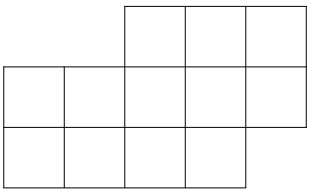
\includegraphics[width=0.3\textwidth]{B36-3}
\end{figure}

%
\prob{B37-1}
집합 \(U=\{1,2,3,4,5\}\)에 대해 \(A\subset U\), \(B\subset U\)를 만족시키는 순서쌍 \((A,B)\)의 개수를 구하시오.
\bigskip\bigskip\bigskip\bigskip\bigskip\bigskip\bigskip\bigskip

%
\prob{B37-2}
집합 \(U=\{1,2,3,4,5\}\)의 두 부분집합 \(A\), \(B\)에 대해서 \(A\subset B\)를 만족하는 순서쌍 \((A,B)\)의 개수를 구하시오.
\bigskip\bigskip\bigskip\bigskip\bigskip\bigskip\bigskip\bigskip

%
\prob{B37-3}
집합 \(U=\{1,2,3,4,5\}\)의 두 부분집합 \(A\), \(B\)에 대해서 \(A\cap B=\{1\}\)를 만족하는 순서쌍 \((A,B)\)의 개수를 구하시오.
\bigskip\bigskip\bigskip\bigskip\bigskip\bigskip\bigskip\bigskip

%
\prob{B37-4}
집합 \(U=\{1,2,3,4,5\}\)의 두 부분집합 \(A\), \(B\)에 대해서 \(A\cup B=\{1,2,3,4\}\), \(A\cap B=\{2\}\) 를 만족하는 순서쌍 \((A,B)\)의 개수를 구하시오.
\bigskip\bigskip\bigskip\bigskip\bigskip\bigskip\bigskip\bigskip

%
\prob{B38-1}
집합 \(\{1,2,3\}\)에서 집합 \(\{1,2,3\}\)로의 함수 중에서 다음 조건을 만족시키는 함수 \(f\)의 개수는?
\begin{enumerate}[(가)]
\item
함수 \(f\)의 치역의 원소의 개수는 \(2\)이다.
\item
합성함수 \(f\circ f\)의 치역의 원소의 개수는 \(1\)이다.
\end{enumerate}
\bigskip\bigskip\bigskip\bigskip\bigskip\bigskip\bigskip\bigskip

%%
%\prob{B38-2}
%집합 \(\{1,2,3,4\}\)에서 집합 \(\{1,2,3,4\}\)로의 함수 중에서 다음 조건을 만족시키는 함수 \(f\)의 개수는?
%\begin{enumerate}[(가)]
%\item
%함수 \(f\)의 치역의 원소의 개수는 \(3\)이다.
%\item
%합성함수 \(f\circ f\)의 치역의 원소의 개수는 \(2\)이다.
%\end{enumerate}

%
\prob{A40-1}
집합 \(\{1,2,3,4\}\)에서 집합 \(\{1,2,3,4\}\)로의 함수 중에서 다음 조건을 만족시키는 함수 \(f\)의 개수는?
\begin{enumerate}[(가)]
\item
함수 \(f\)는 일대일 대응이다.
\item
모든 \(a\in\{1,2,3,4\}\)에 대해 \((f\circ f)(a)\neq a\)이다.
\end{enumerate}
\end{document}